\documentclass[10pt,twocolumn]{article}

\usepackage[T1]{fontenc}
\usepackage[utf8]{inputenc}
\usepackage{lmodern}
\usepackage{microtype}
\usepackage[margin=0.68in,columnsep=0.25in]{geometry}
\usepackage{amsmath,amssymb,amsthm,mathtools}
\usepackage{booktabs}
\usepackage{array}
\usepackage{graphicx}
\usepackage{float}
\usepackage{xcolor}
\usepackage{enumitem}
\usepackage{listings}
\usepackage{tikz}
\usetikzlibrary{arrows.meta,positioning,fit}
\usepackage{fancyhdr}
\usepackage{titlesec}
\usepackage[hidelinks]{hyperref}

\definecolor{ink}{HTML}{152238}
\definecolor{accent}{HTML}{1F5F8B}
\definecolor{soft}{HTML}{EEF4F8}
\definecolor{codebg}{HTML}{F5F7F9}
\definecolor{codegreen}{HTML}{2E6B4E}

\hypersetup{
  colorlinks=true,
  linkcolor=accent,
  citecolor=accent,
  urlcolor=accent,
  pdftitle={A Kernel-Checked Proof of Fuglede's Conjecture for the Cyclic Group Z/180Z},
  pdfauthor={Javier Emilio Bazán Sanchez}
}

\pagestyle{fancy}
\fancyhf{}
\fancyhead[L]{\footnotesize Bazán Sanchez}
\fancyhead[R]{\footnotesize Fuglede's conjecture in $\mathbb Z/180\mathbb Z$}
\fancyfoot[C]{\thepage}
\renewcommand{\headrulewidth}{0.35pt}

\setlength{\parindent}{1em}
\setlength{\parskip}{0pt}
\setlist{nosep,leftmargin=*}
\raggedbottom
\titleformat{\section}{\color{ink}\Large\bfseries}{\thesection}{0.65em}{}
\titleformat{\subsection}{\large\bfseries}{\thesubsection}{0.65em}{}
\titlespacing*{\section}{0pt}{1.5ex plus 0.4ex minus 0.2ex}{0.7ex}
\titlespacing*{\subsection}{0pt}{1.2ex plus 0.3ex minus 0.2ex}{0.5ex}

\newtheorem{theorem}{Theorem}
\newtheorem{proposition}[theorem]{Proposition}
\newtheorem{lemma}[theorem]{Lemma}
\theoremstyle{definition}
\newtheorem{definition}[theorem]{Definition}
\theoremstyle{remark}
\newtheorem{remark}[theorem]{Remark}

\newcommand{\Z}{\mathbb Z}
\newcommand{\Zmod}[1]{\Z/#1\Z}
\newcommand{\mask}{m_A}
\newcommand{\lean}{\textsc{Lean}}

\lstdefinelanguage{Lean}{
  morekeywords={theorem,def,noncomputable,namespace,end,by,exact,intro,
    import,where,structure,abbrev,if,then,else,match,with,fun},
  sensitive=true,
  morecomment=[l]{--},
  morecomment=[s]{/-}{-/},
  morestring=[b]"
}
\lstset{
  language=Lean,
  basicstyle=\ttfamily\scriptsize,
  keywordstyle=\color{accent}\bfseries,
  commentstyle=\color{codegreen},
  backgroundcolor=\color{codebg},
  frame=single,
  rulecolor=\color{black!15},
  breaklines=true,
  columns=fullflexible,
  keepspaces=true,
  showstringspaces=false,
  xleftmargin=0.3em,
  xrightmargin=0.3em,
  aboveskip=0.6em,
  belowskip=0.6em
}

\begin{document}

\twocolumn[
\begin{@twocolumnfalse}
  \begin{center}
    {\color{ink}\LARGE\bfseries
      A Kernel-Checked Proof of Fuglede's Conjecture\\[-1mm]
      for the Cyclic Group $\Z/180\Z$\par}
    \vspace{0.8em}
    {\large Javier Emilio Bazán Sanchez\par}
    \vspace{0.25em}
    {\normalsize Facultad de Ciencias, Universidad Nacional Autónoma de México (UNAM)\par}
    {\normalsize \href{mailto:bazan@ciencias.unam.mx}{bazan@ciencias.unam.mx}\par}
    \vspace{0.6em}
    {\small August 2026\par}
  \end{center}

  \begin{minipage}{0.94\textwidth}
  \small
  \textbf{Abstract.}
  This article gives a machine-checked proof of both directions of Fuglede's conjecture
  for the cyclic group $\Z/180\Z$: a finite subset is spectral if and only if
  it tiles by translation.  Spectrality is encoded exactly by cyclotomic
  divisibility of the integer mask polynomial, and tiling is bijectivity of
  the addition map.  The spectral-to-tiling direction ends in a cardinality
  $30$ classification.  Its marginal audit compresses $16{,}796$ literal
  pairs to $213$ profile cells, refutes $16{,}574$ pairs by exact integer
  coefficients, and links the remaining $222$ to explicit catalogue
  witnesses; a common-frame certificate checks the coupled Gram data.  For
  the converse, an exact Fourier zero-cover theorem reduces all tilings to
  their eighteen possible cardinalities.  Structural closures, quotient
  descent, and a six-point theorem in $\Z/36\Z$ discharge those cases; the
  last thirty-point case is obtained by dilating its six-point complement,
  descending to $\Z/36\Z$, and lifting a six-frequency set through five
  fibres.  Lean~4 and \texttt{leanchecker} replay the final biconditional with
  only \texttt{propext}, \texttt{Classical.choice}, and \texttt{Quot.sound}.
  The complete Lean dependency closure accompanies the article, together with
  the supplemental certificates, deterministic generators, and manifests used
  for the largest spectral-to-tiling branch.
  \end{minipage}
  \vspace{1.1em}
  \hrule
  \vspace{1.2em}
\end{@twocolumnfalse}
]

\section{Introduction}

Fuglede's conjecture relates two rigid structures: a set that admits an
orthogonal basis of characters and a set that tiles its ambient group by
translations.  In Euclidean spaces the unrestricted conjecture is false in
high dimension, while important finite and one-dimensional cases retain a
rich arithmetic structure~\cite{Fuglede1974,Tao2004,DutkayLai2014}.  Finite
cyclic groups are especially useful because Fourier vanishing can be encoded
by divisibility of integer mask polynomials by cyclotomic
polynomials~\cite{CovenMeyerowitz1999}.  This
turns analytic orthogonality into an exact, checkable statement about
polynomials and roots of unity~\cite{LamLeung2000,Malikiosis2022}.

Among the established cyclic families are groups of order $p^nq$, $pqr$,
$p^2qr$, and $pqrs$~\cite{MalikiosisKolountzakis2017,Shi2019,Somlai2023,
KissMalikiosisSomlaiVizer2022}; group-ring methods also treat
$p^nqr$~\cite{Zhang2022}.  A closer recent result proves the
spectral-to-tiling direction for $\Z_{p^2q^2r}$ under the size condition
$p^2q^2<r$~\cite{FallonKissMayeliSomlai2026}.  At order $180$, however,
this condition reads $36<5$ and therefore does not apply.  The reverse
direction is related to broader results on three-prime integer tilings and
the Coven--Meyerowitz conditions~\cite{LabaLondnerEven2024}.  The present
work gives a self-contained kernel-checked proof specialized to order $180$;
it makes no claim about arbitrary moduli.

This article reports a complete formal proof of both directions for
$G=\Zmod{180}$, where
\[
180=2^2\cdot 3^2\cdot 5.
\]
The spectral-to-tiling direction is driven by structural reductions and a
finite classification.  Its difficult residual case has $|A|=30$ and
requires both a marginal classification and compatibility of a five-row Gram
configuration.  The converse starts from the exact Fourier characterization
of a tiling pair, resolves all possible divisor cardinalities, and closes its
last thirty-point case by descent to $\Zmod{36}$.

Every finite computation reaches the kernel as an ordinary Lean declaration,
rather than remaining an oracle beside the proof.  For the largest generated
V97 sub-DAG, deterministic scripts emit those declarations and hash manifests
fail closed if sources, catalogues, witness locations, or import order change.
The rest of the theorem is likewise committed as checkable Lean source.  No
floating-point calculation enters the theorem.

\subsection*{Contribution}

The formal development establishes the finite cyclic Fuglede conjecture at
order $180$.

\begin{theorem}[Kernel-checked Fuglede theorem at order $180$]\label{thm:main}
For every $A\subseteq\Zmod{180}$, the following conditions are equivalent:
\begin{enumerate}[label=\textup{(\roman*)}]
  \item $A$ tiles $\Zmod{180}$ by translation;
  \item $A$ admits an orthogonal basis of characters.
\end{enumerate}
Equivalently, there is a finite set $B$ for which the addition map
$A\times B\to\Zmod{180}$ is bijective if and only if there is a finite set
$L$ that is an exact cyclotomic spectrum for $A$.
\end{theorem}

In the repository, Theorem~\ref{thm:main} is the declaration
\texttt{Fuglede.z180\_tiles\_iff\_spectral}.

\section{The exact finite formulation}

For $A\subseteq\Zmod{N}$, choose the standard representatives
$a\in\{0,\ldots,N-1\}$ and define the mask polynomial
\[
  \mask(X)=\sum_{a\in A}X^a\in\Z[X].
\]
For $d\in\Zmod N$, let
\[
  \operatorname{ord}_N(d)=\frac{N}{\gcd(N,d)}.
\]
The formal predicate \texttt{CyclotomicZero} requires
\[
  \Phi_{\operatorname{ord}_N(d)}(X)\mid \mask(X)
  \quad\text{in }\Z[X].
\]
This is the exact algebraic certificate used for Fourier vanishing at
frequency $d$.

\begin{definition}[Exact cyclotomic spectrum]
A finite set $L\subseteq\Zmod N$ is a cyclotomic spectrum for $A$ if
$A\ne\varnothing$, $|A|=|L|$, and for every two distinct
$\ell_1,\ell_2\in L$,
\[
  \Phi_{\operatorname{ord}_N(\ell_1-\ell_2)}\mid \mask.
\]
\end{definition}

This predicate is not a substitute for the usual analytic definition.  Let
$\chi_N$ be the standard injective additive character of $\Zmod N$ and define
the unnormalised Fourier coefficient
\[
  \widehat{\mathbf 1_A}(d)=\sum_{a\in A}\chi_N(ad).
\]
The formalization proves the exact equivalence
\begin{equation}\label{eq:fourier-bridge}
  \Phi_{\operatorname{ord}_N(d)}\mid \mask
  \quad\Longleftrightarrow\quad
  \widehat{\mathbf 1_A}(d)=0.
\end{equation}
It follows that \texttt{CyclotomicSpectrum} is equivalent to the ordinary
pairwise Fourier-orthogonality condition.  Because $|A|=|L|$ and
$A\ne\varnothing$, the Fourier evaluation matrix is square with nonzero,
orthogonal columns; its characters therefore form an orthogonal basis on
$A$.  Lean also proves the dual spectrum statement by converting column
orthogonality into row orthogonality.  Thus Theorem~\ref{thm:main} assumes the
standard finite notion of spectrality, expressed in an exact algebraic form.

The tiling predicate is deliberately independent of Fourier analysis.
For finite sets $A,B\subseteq G$, let
\[
  f_{A,B}:A\times B\longrightarrow G,
  \qquad f_{A,B}(a,b)=a+b.
\]
Lean defines
\[
  \operatorname{Tiles}(A,B)
  \quad\Longleftrightarrow\quad
  f_{A,B}\text{ is bijective}.
\]
Thus the conclusion includes both existence and uniqueness of each
representation.  In particular, it implies $|A||B|=|G|$.

In ASCII notation, the public endpoint has the following type; the two imported
endpoints supply its proof.

\begin{lstlisting}
theorem z180_tiles_iff_spectral
    (A : Finset (ZMod 180)) :
    Iff
      (Exists fun B : Finset (ZMod 180) => Tiles A B)
      (Exists fun L : Finset (ZMod 180) =>
        CyclotomicSpectrum 180 A L)
\end{lstlisting}

The two imported endpoints contain the substantive work.  The
spectral-to-tiling classification is described first, followed by the
tiling-to-spectral reduction.

\section{The spectral-to-tiling direction}

Figure~\ref{fig:architecture} shows the dependency structure of the
computationally harder implication.  The global
reduction isolates the cardinality-$30$ obstruction.  That obstruction has a
projective/marginal component (V97) and a coupled common-frame component
(V95).  V81 turns their catalogue into the global theorem, and V96 supplies
the two certificates unconditionally.

\begin{figure*}[t]
\centering
\resizebox{0.96\textwidth}{!}{%
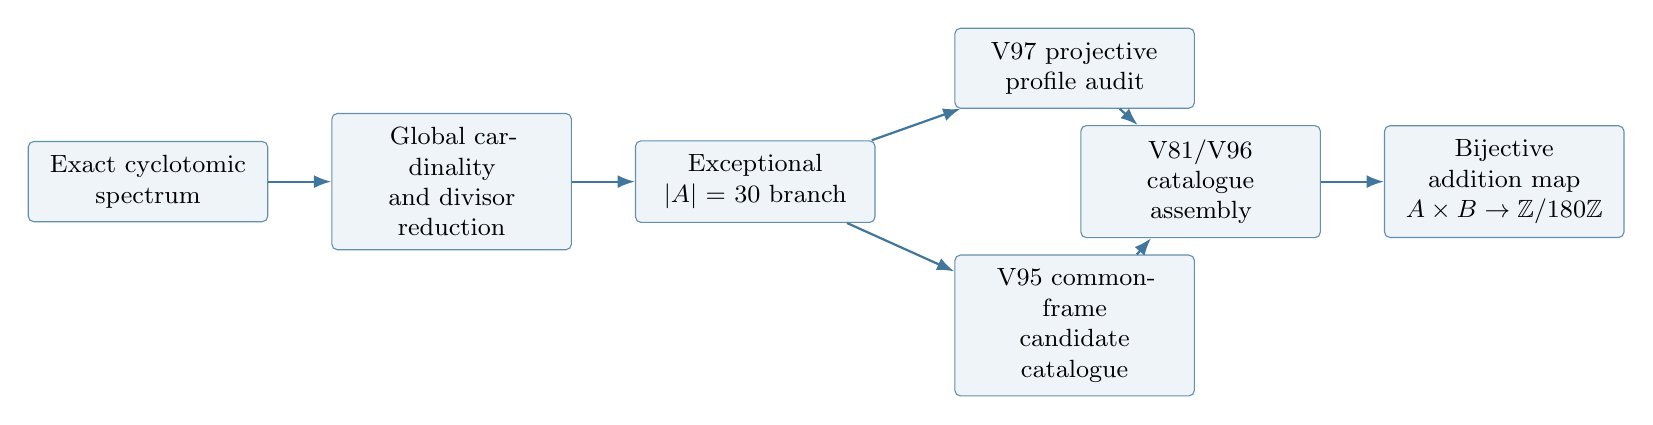
\begin{tikzpicture}[
  node distance=7mm and 8mm,
  box/.style={draw=accent!70, rounded corners=2pt, fill=soft,
    align=center, inner xsep=7pt, inner ysep=5pt,
    text width=2.55cm, font=\small},
  arr/.style={-{Latex[length=2.2mm]}, thick, draw=accent!85}
]
\node[box] (spec) {Exact cyclotomic\\spectrum};
\node[box, right=of spec] (global) {Global cardinality\\and divisor reduction};
\node[box, right=of global] (k30) {Exceptional\\$|A|=30$ branch};
\node[box, above right=4mm and 10mm of k30] (v97) {V97 projective\\profile audit};
\node[box, below right=4mm and 10mm of k30] (v95) {V95 common-frame\\candidate catalogue};
\node[box, right=26mm of k30] (v96) {V81/V96 catalogue\\assembly};
\node[box, right=of v96] (tile) {Bijective addition map\\$A\times B\to\Zmod{180}$};
\draw[arr] (spec) -- (global);
\draw[arr] (global) -- (k30);
\draw[arr] (k30) -- (v97);
\draw[arr] (k30) -- (v95);
\draw[arr] (v97) -- (v96);
\draw[arr] (v95) -- (v96);
\draw[arr] (v96) -- (tile);
\end{tikzpicture}
}
\caption{High-level structure of the checked proof.  V97 and V95 are
independent finite certificates joined only at catalogue assembly.}
\label{fig:architecture}
\end{figure*}

The version labels in Figure~\ref{fig:architecture} are immutable module
suffixes: V97 is the projective-profile audit, V95 the common-frame
certificate, V83 their catalogue interface, V81 the global reduction, and V96
the unconditional spectral-to-tiling endpoint.

\subsection{The global reduction}

The surrounding library converts the spectrum hypothesis into exact
cyclotomic zero data, applies cardinality and divisor sieves, and closes the
nonexceptional branches.  Sets of size greater than $90$ are handled by the
upper-half reduction.  At size at most $90$, projection to complementary
factors restricts the cardinality to a divisor of $180$ or to
\[
  7,8,11,13,14,16,17,19,21,24,27,33.
\]
Kernel-checked nondivisor arguments eliminate all entries in this list except
the intermediate $24$ and $33$ branches.  The divisor reduction and subsequent
closures discharge the residual sizes $6,10,12,18$; separate arguments close
$33$ and exclude $24$.  The master conditional theorem consequently asks
only for a closure at cardinality $30$.  The module
\texttt{Z180K30CatalogueMasterClosureV81} packages this interface:
a complete exceptional catalogue implies the spectral-to-tiling theorem for
all cardinalities.

This separation is valuable both mathematically and formally.  The general
Fourier and tiling lemmas do not depend on the large finite catalogue, while
the catalogue proof sees a small and rigid normalized state space.

\subsection{Projective normalization and ordered differences}

The exceptional reduction starts from balanced cardinality-$30$ data and
passes to five six-point row fibres and one six-point column fibre in
$\Zmod{36}$.  Fixing a column fibre gives five $6\times6$ Fourier blocks.
Let $V$ denote its six residues and $U_0,\ldots,U_4$ the five row patterns; a
marginal check below uses one such row and abbreviates it by $U$.
The projective-cover alternative orients the pair so that $V$ is the side
whose differences have a nontrivial common divisor
\[
  d=\gcd\bigl(36,\{v-v':v,v'\in V\}\bigr).
\]
Validity of the six-point sets bounds $d$ by $6$, while the two-class
condition on $U$ eliminates $d=1,2$.  Lean therefore proves
$d\in\{3,4,6\}$.  Thus $U$, $V$, and $d$ below are normalized fibre data
forced by the exceptional branch, not new assumptions.

The projective branch works with six-element subsets of $\Zmod{36}$.  For a
list $S$, define its ordered-difference list
\[
  \Delta(S)=\bigl((x-y)\bmod 36\bigr)_{(x,y)\in S^2}.
\]
Diagonal terms are retained.  The scalar Gram coefficient used by the audit
can be written as the bilinear sum
\begin{equation}\label{eq:bilinear}
  \Gamma(U,V)
  =\sum_{a\in\Delta(U)}\sum_{b\in\Delta(V)}\zeta_0(ab),
\end{equation}
where $\zeta_0$ is the exact integer-valued coefficient extracted from the
cyclotomic representation.  Lean proves Equation~\eqref{eq:bilinear} by
unfolding the Gram trace.  Exchanging the two finite sums and using
$ab=ba$ proves
\[
  \Gamma(U,V)=\Gamma(V,U).
\]
This symmetry removes a duplicated orientation from the finite audit.

For a supported divisor $d\in\{3,4,6\}$, every difference on the normalized
$V$-side is a multiple of $d$.  The $U$-profile stores the responses
\[
  K_{d,U}(t)=\sum_{a\in\Delta(U)}\zeta_0(at),
  \qquad 0\le t<36,
\]
with zero outside the multiples of $d$.  The $V$-profile is the sorted list
$\Delta(V)$, which is a canonical representation of its histogram.  A proved
compression lemma states
\begin{equation}\label{eq:profile}
  \Gamma(U,V)=\sum_{b\in\Delta(V)}K_{d,U}(b).
\end{equation}
Sorting changes no sum because Lean carries an explicit permutation proof.
The use of a sorted list rather than an unverified hash is important: profile
equality is itself checked in the kernel.

\subsection{The finite profile census}

The normalized literal universe contains $16{,}796$ distinct pairs.  Grouping
by the two exact profiles produces the much smaller table in
Table~\ref{tab:census}.

\begin{table}[H]
\centering
\caption{Authenticated projective-profile census.}
\label{tab:census}
\small
\begin{tabular}{@{}rrrrr@{}}
\toprule
$d$ & $U$ profiles & $V$ profiles & cells & positive pairs \\
\midrule
3 & 5 & 35 & 175 & 42 \\
4 & 4 & 7  & 28  & 0 \\
6 & 10 & 1 & 10 & 180 \\
\midrule
Total & 19 & 43 & 213 & 222 \\
\bottomrule
\end{tabular}
\end{table}

The exceptional spectral argument determines the six eigenvalues of each Gram
block: one is $30$, one is $6$, and four are zero.  Consequently its exact
trace-square target is
\[
  \operatorname{tr}(G^2)=30^2+6^2=936.
\]
Each profile cell evaluates the corresponding integer coefficient.  A value
different from $936$ refutes every pair in that cell.  This eliminates
$16{,}574$ pairs.  A cell attaining $936$ is not accepted merely because the
total count is plausible:
each of the remaining $222$ literal pairs carries an exact pointer into one of
the certified V87 witness shards.  Lean checks the shard index, witness index,
divisor, normalization, and the literal $U,V$ values.  The surviving counts
$42+180$ therefore express a set equality, not a probabilistic or numerical
match.

The profile compression was also essential for proof engineering.  Expanding
the original pairwise Gram computation retained millions of repeated root-of-
unity reductions and exceeded practical memory limits.  Equations
\eqref{eq:bilinear}--\eqref{eq:profile} move the repeated work into a small set
of reusable profiles without changing the certified proposition.

\subsection{The common-frame branch}

The marginal catalogue is insufficient by itself: five row configurations
must be compatible with the same column frame.  The V95 branch handles this
coupled condition.

For a fixed normalized column orbit $o$, let $c_{e,k}(W,V_o)$ denote the exact
integer coefficient at Gram entry $e$ and cyclotomic coordinate $k$.  The row
signature is a short list
\[
  \sigma_o(W)=\bigl(c_{e_j,k_j}(W,V_o)\bigr)_{j=1}^{t},
  \qquad t\in\{0,1,2\},
\]
where the selected entries depend only on $o$.  The coupled star condition
retains the five signatures
$\bigl(\sigma_o(U_0),\ldots,\sigma_o(U_4)\bigr)$ in one affine frame and
requires their selected coordinates to sum to zero.  It also records that each
pair $(U_i,V_o)$ has trace-square $936$ and that the five Gram matrices sum to
the diagonal target with value $30$.

First, an orbit-frame extractor writes the normalized column as one affine
image with a unit and a translation.  The same unit is then applied to every
row.  Covariance lemmas transport the selected coordinates of all five rows
into this common frame.  Second, a trace classifier identifies the only
compatible row orbit.
Finally, a bounded affine table supplies a valid candidate with the same exact
star signature.  Permutation invariance transports the candidate from the
representative to the original row.

The V83 catalogue interface returns both the five candidates and proofs that
their exact coordinates realize the required star.  The finite affine leaves,
their aggregate, and the final common-frame module are all replayed separately.

\subsection{Catalogue assembly}

The V97 normalization gives marginal coverage.  The V95 framed-star object
gives the coupled witness.  V83 combines them into complete exceptional
catalogue data; V81 converts that data into the global cardinality-$30$
closure and then invokes the previously completed cardinality reduction.  V96
is the final three-import wrapper joining these components.

\section{The tiling-to-spectral direction}

The converse uses the same exact Fourier language but a different proof
architecture.  For a tiling pair $(A,B)$ in a finite cyclic group, convolution
and character orthogonality give
\begin{equation}\label{eq:zero-cover}
\begin{aligned}
 \operatorname{Tiles}(A,B)\Longleftrightarrow{}&
 |A||B|=N\ \text{ and}\\
 &\forall d\ne0,\quad \bigl(\widehat{\mathbf 1_A}(d)=0\\
 &\hspace{6.3em}\text{or }\widehat{\mathbf 1_B}(d)=0\bigr).
\end{aligned}
\end{equation}
Lean proves both implications, including Fourier inversion from the right-hand
side back to uniqueness of representations.  Equation~\eqref{eq:fourier-bridge}
then converts this zero cover to cyclotomic divisibility.

The cardinality identity in Equation~\eqref{eq:zero-cover} leaves exactly the
eighteen positive divisors of $180$.  The reduction closes them in stages,
with the final two cases isolated as $|A|=6$ and $|A|=30$.
Table~\ref{tab:converse-cases} summarizes the mechanisms used for all cases.

\begin{table}[t]
\centering
\caption{Cardinality closures for tiling-to-spectrality.}
\label{tab:converse-cases}
\small
\begin{tabular}{@{}p{0.30\columnwidth}p{0.62\columnwidth}@{}}
\toprule
Cardinalities & Main mechanism \\
\midrule
$1,2,3,180$ & Endpoint and direct character arguments \\
$4,5,9$ & Prime-power allocation \\
$60,90$ & Small-complement Fourier construction \\
$20,36,45$ & Exact cyclotomic forcing \\
$10,12,15,18$ & Quotient descent and lifted spectra \\
$6,30$ & Six-point forcing in $\Zmod{36}$ \\
\bottomrule
\end{tabular}
\end{table}

The six-point theorem in $\Zmod{36}$ is the reusable core.  For a $6\times6$
tiling, the zero cover allocates exactly one of the orders $2,4$ and one of the
orders $3,9$ to each factor.  Previously checked forcing lemmas turn the
remaining orders into one of five explicit difference patterns, each of which
supplies a six-frequency spectrum.  A six-point tile in $\Zmod{180}$ descends
injectively modulo $36$ and its spectrum lifts by multiplying frequencies by
five.

For the last case, suppose $|A|=30$.  Its tiling complement has six elements.
Multiplication by five preserves that complement as a tiling factor, while
reduction modulo $36$ sends it injectively to a six-point set $C$.  An explicit
six-frequency set $Q\subseteq\Zmod{36}$ is chosen so that the Fourier transform
of $C$ is nonzero on every nonzero difference from $Q$.  The full preimage
$L$ of $Q$ in $\Zmod{180}$ has $5\cdot6=30$ elements.  The zero-cover property
forces the Fourier transform of $A$ to vanish on every nonzero difference in
$L$, so $L$ is a spectrum for $A$.

These constructions form the V12 tiling-to-spectral endpoint.  Combining it
with the V96 spectral-to-tiling endpoint yields the public theorem
\texttt{z180\_tiles\_iff\_spectral} without any additional finite search.

\section{Formal verification and trust}

The development uses Lean~4.31.0 and a pinned mathlib revision.  Lean and
mathlib provide a small trusted kernel and a large reusable mathematical
library~\cite{deMouraUllrich2021,Mathlib2020}.  The release adopts the following
policy.

\paragraph{Exact arithmetic.}
Mask polynomials have integer coefficients.  Finite Gram computations reduce
to integer lists and exact cyclotomic coefficients.  There is no floating-
point tolerance and no numerical root approximation.

\paragraph{Untrusted generation, trusted checking.}
Python and PowerShell generate literal definitions, theorem statements, and
replay schedules.  They are convenience tools, not part of the logical trust
base.  Every generated declaration is elaborated by Lean.  Structural roots
are replayed again by \texttt{leanchecker}.

\paragraph{No proof escape hatches.}
The complete 2,411-module dependency closure of the final biconditional
contains no \texttt{sorry}, \texttt{admit}, project-defined \texttt{axiom},
\texttt{native\_decide}, or \texttt{unsafe}.  In the large V97 sub-DAG,
ordinary decisions are deliberately kept small; larger statements are split
into bounded leaves and composed with proved list and permutation lemmas.

\paragraph{Fail-closed provenance.}
The master manifest authenticates 946 modules in a unique topological order,
including an external algebraic closure of 757 modules.  It pins child
manifests, generators, catalogue inputs, the order of 66 witness shards, and
the $16{,}796/213/222$ census.  Source drift causes authentication to stop
before Lean is launched.

\paragraph{Axiom report.}
For both catalogue completeness and the final theorem, Lean prints exactly
\[
  [\texttt{propext},\ \texttt{Classical.choice},\ \texttt{Quot.sound}].
\]
These are the standard classical and quotient principles used by mathlib; no
problem-specific axiom appears.

\section{Reproducing the artifact}

The repository contains the exact transitive Lean source closure of the final
theorem, the pinned toolchain, the article, and supplementary provenance for
the large V97 certificate.  The public artifact is available at
\url{https://github.com/asim-v/fuglede-z180-formal}.  The shortest kernel
replay is:

\noindent\begin{minipage}{\dimexpr\columnwidth-2\fboxsep-2\fboxrule\relax}
\begin{lstlisting}[language={},basicstyle=\ttfamily\scriptsize]
cd fuglede_lean
lake update
lake exe cache get
lake build '+Fuglede.Z180FugledeTheorem:olean'
lake env leanchecker -v Fuglede.Z180FugledeTheorem
cd ..
\end{lstlisting}
\end{minipage}

Every proof-relevant finite certificate is an ordinary Lean source file in
that import closure; no external solver or Python program is trusted by the
final theorem.  As an additional provenance check for the largest generated
sub-DAG, run:

\begin{lstlisting}[language={},basicstyle=\ttfamily\scriptsize]
python scripts/generate_z180_k30_projective_profile_audit_v97.py
\end{lstlisting}

This command authenticates the V97 sources and manifest.  The serialized
PowerShell runner provides a module-by-module replay under a fixed memory cap.

\section{Scope and interpretation}

Theorem~\ref{thm:main} is intentionally precise.

\begin{itemize}
  \item It proves both spectral-to-tiling and tiling-to-spectral for
    $\Zmod{180}$.
  \item Equation~\eqref{eq:fourier-bridge} identifies the exact cyclotomic
    predicate with the usual finite Fourier definition; no approximate
    vanishing is assumed.
  \item Tiling means unique representation under addition, not merely a
    cardinality or covering condition.
  \item The theorem concerns one finite cyclic group.  It is not a theorem for
    arbitrary moduli, arbitrary finite abelian groups, or Euclidean spaces.
  \item The large finite leaves are proof terms checked by Lean and are best
    inspected and replayed as code.
\end{itemize}

This distinction is more than cautious wording.  Formal verification certifies
that the encoded theorem follows from its definitions; it does not replace the
mathematical task of stating those definitions faithfully.  For that reason
the exact Lean predicates and the public endpoint are included explicitly.

\section{Conclusion}

Fuglede's conjecture holds for the finite cyclic group $\Zmod{180}$.  The two
directions require complementary ideas.  Spectral-to-tiling uses a structured
finite certificate whose difficult cardinality-$30$ branch separates marginal
profile data from coupled common-frame data.  Ordered-difference profiles
compress its marginal audit to 213 exact cells, and explicit witness pointers
prevent positive cases from being accepted by count alone.  Tiling-to-spectral
uses an exact Fourier zero cover, cardinality reduction, and quotient descent;
its final case lifts a six-frequency construction from $\Zmod{36}$.

The final declaration merely joins these independently checked endpoints, but
its complete transitive source closure is public: definitions, algebraic
identities, finite tables, generated proof terms, hashes, and replay commands
are all exposed.  The result is therefore both a theorem about a concrete
cyclic group and a reproducible case study in turning large finite
harmonic-analysis arguments into kernel-checked mathematics.

\section*{Acknowledgements}

The formalization uses Lean and the mathlib library.  The author thanks the
developers and maintainers of these open-source projects.

\begingroup
\footnotesize
\bibliographystyle{abbrv}
\bibliography{references}
\endgroup

\end{document}
